\documentclass[11pt,letterpaper]{article}
%\documentclass[11pt,letterpaper]{exam}
\usepackage[latin1]{inputenc}
\usepackage[left=3.00cm, right=3.00cm, top=3.00cm, bottom=3.00cm]{geometry}

\usepackage{amsmath}
%\usepackage{amsthm}
%\usepackage{cancel}
\usepackage{mathtools}
%\DeclarePairedDelimiter\ceil{\lceil}{\rceil}
%\DeclarePairedDelimiter\floor{\lfloor}{\rfloor}

\usepackage{fancyhdr}
\pagestyle{fancy}

\usepackage{color}
%\usepackage{xcolor}
%\usepackage{graphicx}
\usepackage{caption}
%\definecolor{acolour}{rgb}{0,0.0,0}

%\usepackage{url}
\usepackage{listings}
%\usepackage[]{algorithm2e}

\lstset{frame=tb,
	language=Java,
	aboveskip=3mm,
	belowskip=3mm,
	showstringspaces=false,
	%frame=tb,
	columns=flexible,
	basicstyle={\small\ttfamily},
	numbers=none,
	numberstyle=\tiny\color{gray},
	keywordstyle=\color{blue},
	commentstyle=\color{dkgreen},
	stringstyle=\color{mauve},
	breaklines=true,
	breakatwhitespace=true,
	tabsize=3
}

\newcounter{nalg}[section] % defines algorithm counter for chapter-level
\renewcommand{\thenalg}{\thechapter .\arabic{nalg}} %defines appearance of the algorithm counter
\DeclareCaptionLabelFormat{algocaption}{Algorithm \thenalg} % defines a new caption label as Algorithm x.y

\lstnewenvironment{algorithm}[1][] %defines the algorithm listing environment
{   
	\refstepcounter{nalg} %increments algorithm number
	\captionsetup{labelformat=algocaption,labelsep=colon} %defines the caption setup for: it uses label format as the declared caption label above and makes label and caption text to be separated by a ':'
	\lstset{ %this is the stype
		mathescape=true,
		frame=tB,
		numbers=left, 
		numberstyle=\tiny,
		basicstyle=\scriptsize, 
		keywordstyle=\color{blue}\bfseries\em,
		keywords={,input, output, return, datatype, function, in, if, else, foreach, while, begin, end, true, false, int, for, then, } %add the keywords you want, or load a language as Rubens explains in his comment above.
		numbers=left,
		xleftmargin=.02\textwidth,
		#1 % this is to add specific settings to an usage of this environment (for instnce, the caption and referable label)
	}
}
{}

\author{Simon Zheng\\260744353}
\title{Homework 1}
\date{January 30$^{\textnormal{th}}$, 2018}
\lhead{COMP 424}
%\chead{Homework $$}
\rhead{Artificial Intelligence}

\begin{document}
	\maketitle
	\thispagestyle{fancy}
	
	\section{Six-Puzzle}
		\subsection{}
		\begin{figure}[ht]
			\centering
			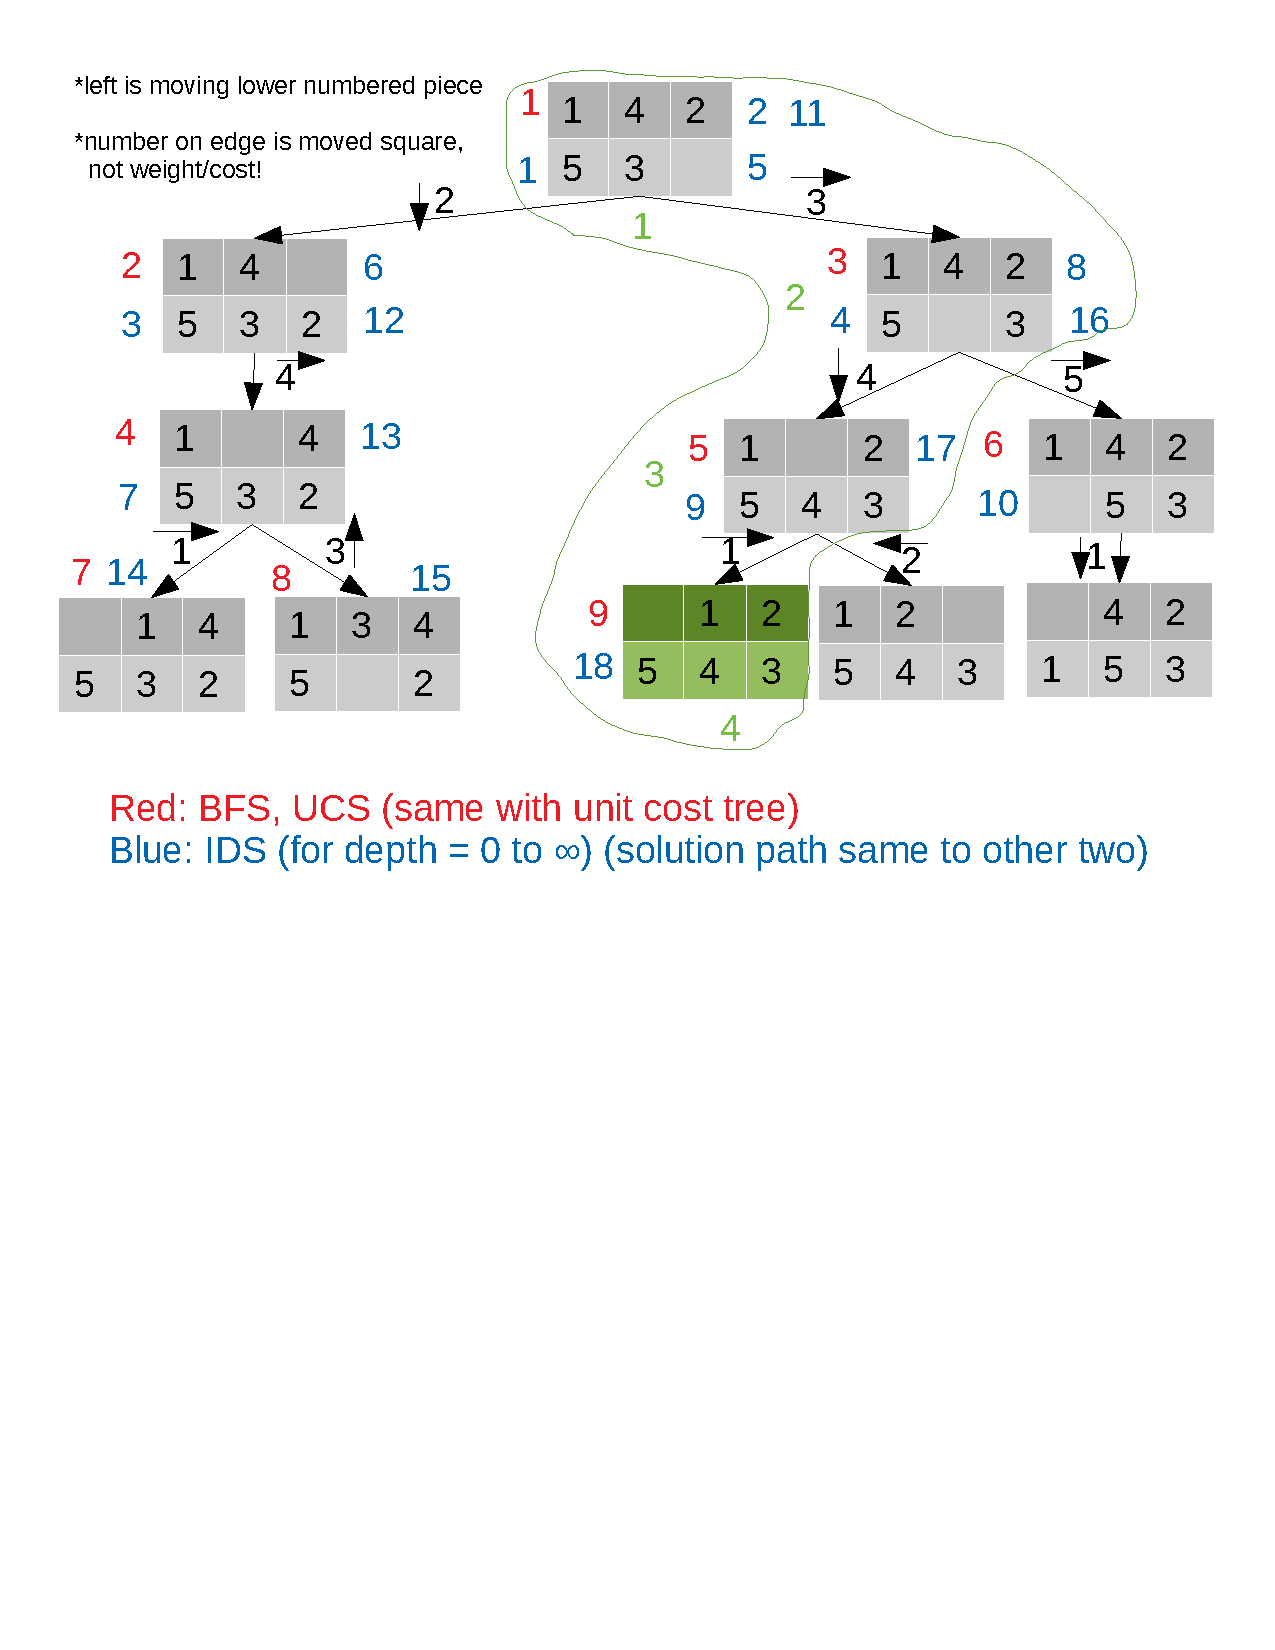
\includegraphics[height=300px,width=400px,trim={0 360px 0 0},clip]{q1.pdf}
			\linespread{0.8}\caption{Counter-example.}
		\end{figure}
		
	\section{Search algorithms}
	    \subsection{a)}
	    
	    \subsection{b)}
	    True.
	    If you run UCS on a graph with unit costs (or equal costs), then it will behave like BFS, thus BFS is a special case of UCS with unit costs.
	    The algorithm would not prioritize one child or neighbor over another since the cost is not better or worst for any of them.
	    Instead, the depth would add up equally and thus this UCS would expand the lowest depth nodes first.
	    Thus, the priority queue acts as a normal queue and the algorithm behave as a BFS.
	    
	    \subsection{c)}
	    True.
	    A Best-First Search which uses a heuristic function where it expands the deepest node first behaves like DFS.
	    The heuristic would evaluate the negative depth (from the root node) such that a larger depth has an inferior cost.
	    
	    \subsection{d)}
	    True.
	    We know that an A* Search evaluates which nodes to expand based on a function which calculates the cost and uses a heuristic.
	    As an uninformed search, UCS would simply ignore the heuristic part of the evaluation function.
	    Thus, what we are left with is the cost function, which would simply be a UCS.
	
	\section{Optimization}
	
	\section{Constraint satisfaction}
	    \subsection{a)}
	    \begin{itemize}
            \item Variables: rooks $\{R_1, R_2, ... , R_k\}$ where $R_i = [x_i, y_i]$ (position of the rook on the board)
            \item Domain: $k \leq n^2, \{\forall x_i, y_i | x_i < n \wedge y_i < n \wedge x_i \in \mathbf{N} \wedge y_i \in \mathbf{N}\}$ (position of each rook must be within board and positive integer)
            \item Constraints: $\left|R_i - R_j\right| \neq \left|i - j\right|$ (no two rooks can be on the same diagonal)
        \end{itemize}
        
        \subsection{b)}
        
        
        \subsection{c)}
        
	
\end{document}
